% Options for packages loaded elsewhere
\PassOptionsToPackage{unicode}{hyperref}
\PassOptionsToPackage{hyphens}{url}
%
\documentclass[
]{book}
\usepackage{amsmath,amssymb}
\usepackage{lmodern}
\usepackage{iftex}
\ifPDFTeX
  \usepackage[T1]{fontenc}
  \usepackage[utf8]{inputenc}
  \usepackage{textcomp} % provide euro and other symbols
\else % if luatex or xetex
  \usepackage{unicode-math}
  \defaultfontfeatures{Scale=MatchLowercase}
  \defaultfontfeatures[\rmfamily]{Ligatures=TeX,Scale=1}
\fi
% Use upquote if available, for straight quotes in verbatim environments
\IfFileExists{upquote.sty}{\usepackage{upquote}}{}
\IfFileExists{microtype.sty}{% use microtype if available
  \usepackage[]{microtype}
  \UseMicrotypeSet[protrusion]{basicmath} % disable protrusion for tt fonts
}{}
\makeatletter
\@ifundefined{KOMAClassName}{% if non-KOMA class
  \IfFileExists{parskip.sty}{%
    \usepackage{parskip}
  }{% else
    \setlength{\parindent}{0pt}
    \setlength{\parskip}{6pt plus 2pt minus 1pt}}
}{% if KOMA class
  \KOMAoptions{parskip=half}}
\makeatother
\usepackage{xcolor}
\IfFileExists{xurl.sty}{\usepackage{xurl}}{} % add URL line breaks if available
\IfFileExists{bookmark.sty}{\usepackage{bookmark}}{\usepackage{hyperref}}
\hypersetup{
  pdftitle={Spatial R Exercise 7},
  pdfauthor={Ben Davies},
  hidelinks,
  pdfcreator={LaTeX via pandoc}}
\urlstyle{same} % disable monospaced font for URLs
\usepackage{color}
\usepackage{fancyvrb}
\newcommand{\VerbBar}{|}
\newcommand{\VERB}{\Verb[commandchars=\\\{\}]}
\DefineVerbatimEnvironment{Highlighting}{Verbatim}{commandchars=\\\{\}}
% Add ',fontsize=\small' for more characters per line
\usepackage{framed}
\definecolor{shadecolor}{RGB}{248,248,248}
\newenvironment{Shaded}{\begin{snugshade}}{\end{snugshade}}
\newcommand{\AlertTok}[1]{\textcolor[rgb]{0.94,0.16,0.16}{#1}}
\newcommand{\AnnotationTok}[1]{\textcolor[rgb]{0.56,0.35,0.01}{\textbf{\textit{#1}}}}
\newcommand{\AttributeTok}[1]{\textcolor[rgb]{0.77,0.63,0.00}{#1}}
\newcommand{\BaseNTok}[1]{\textcolor[rgb]{0.00,0.00,0.81}{#1}}
\newcommand{\BuiltInTok}[1]{#1}
\newcommand{\CharTok}[1]{\textcolor[rgb]{0.31,0.60,0.02}{#1}}
\newcommand{\CommentTok}[1]{\textcolor[rgb]{0.56,0.35,0.01}{\textit{#1}}}
\newcommand{\CommentVarTok}[1]{\textcolor[rgb]{0.56,0.35,0.01}{\textbf{\textit{#1}}}}
\newcommand{\ConstantTok}[1]{\textcolor[rgb]{0.00,0.00,0.00}{#1}}
\newcommand{\ControlFlowTok}[1]{\textcolor[rgb]{0.13,0.29,0.53}{\textbf{#1}}}
\newcommand{\DataTypeTok}[1]{\textcolor[rgb]{0.13,0.29,0.53}{#1}}
\newcommand{\DecValTok}[1]{\textcolor[rgb]{0.00,0.00,0.81}{#1}}
\newcommand{\DocumentationTok}[1]{\textcolor[rgb]{0.56,0.35,0.01}{\textbf{\textit{#1}}}}
\newcommand{\ErrorTok}[1]{\textcolor[rgb]{0.64,0.00,0.00}{\textbf{#1}}}
\newcommand{\ExtensionTok}[1]{#1}
\newcommand{\FloatTok}[1]{\textcolor[rgb]{0.00,0.00,0.81}{#1}}
\newcommand{\FunctionTok}[1]{\textcolor[rgb]{0.00,0.00,0.00}{#1}}
\newcommand{\ImportTok}[1]{#1}
\newcommand{\InformationTok}[1]{\textcolor[rgb]{0.56,0.35,0.01}{\textbf{\textit{#1}}}}
\newcommand{\KeywordTok}[1]{\textcolor[rgb]{0.13,0.29,0.53}{\textbf{#1}}}
\newcommand{\NormalTok}[1]{#1}
\newcommand{\OperatorTok}[1]{\textcolor[rgb]{0.81,0.36,0.00}{\textbf{#1}}}
\newcommand{\OtherTok}[1]{\textcolor[rgb]{0.56,0.35,0.01}{#1}}
\newcommand{\PreprocessorTok}[1]{\textcolor[rgb]{0.56,0.35,0.01}{\textit{#1}}}
\newcommand{\RegionMarkerTok}[1]{#1}
\newcommand{\SpecialCharTok}[1]{\textcolor[rgb]{0.00,0.00,0.00}{#1}}
\newcommand{\SpecialStringTok}[1]{\textcolor[rgb]{0.31,0.60,0.02}{#1}}
\newcommand{\StringTok}[1]{\textcolor[rgb]{0.31,0.60,0.02}{#1}}
\newcommand{\VariableTok}[1]{\textcolor[rgb]{0.00,0.00,0.00}{#1}}
\newcommand{\VerbatimStringTok}[1]{\textcolor[rgb]{0.31,0.60,0.02}{#1}}
\newcommand{\WarningTok}[1]{\textcolor[rgb]{0.56,0.35,0.01}{\textbf{\textit{#1}}}}
\usepackage{longtable,booktabs,array}
\usepackage{calc} % for calculating minipage widths
% Correct order of tables after \paragraph or \subparagraph
\usepackage{etoolbox}
\makeatletter
\patchcmd\longtable{\par}{\if@noskipsec\mbox{}\fi\par}{}{}
\makeatother
% Allow footnotes in longtable head/foot
\IfFileExists{footnotehyper.sty}{\usepackage{footnotehyper}}{\usepackage{footnote}}
\makesavenoteenv{longtable}
\usepackage{graphicx}
\makeatletter
\def\maxwidth{\ifdim\Gin@nat@width>\linewidth\linewidth\else\Gin@nat@width\fi}
\def\maxheight{\ifdim\Gin@nat@height>\textheight\textheight\else\Gin@nat@height\fi}
\makeatother
% Scale images if necessary, so that they will not overflow the page
% margins by default, and it is still possible to overwrite the defaults
% using explicit options in \includegraphics[width, height, ...]{}
\setkeys{Gin}{width=\maxwidth,height=\maxheight,keepaspectratio}
% Set default figure placement to htbp
\makeatletter
\def\fps@figure{htbp}
\makeatother
\setlength{\emergencystretch}{3em} % prevent overfull lines
\providecommand{\tightlist}{%
  \setlength{\itemsep}{0pt}\setlength{\parskip}{0pt}}
\setcounter{secnumdepth}{5}
\usepackage{booktabs}
\ifLuaTeX
  \usepackage{selnolig}  % disable illegal ligatures
\fi
\usepackage[]{natbib}
\bibliographystyle{plainnat}

\title{Spatial R Exercise 7}
\author{Ben Davies}
\date{2022-05-12}

\begin{document}
\maketitle

{
\setcounter{tocdepth}{1}
\tableofcontents
}
\hypertarget{getting-started-with-point-patterns}{%
\chapter{Getting started with point patterns}\label{getting-started-with-point-patterns}}

Oftentimes, the geographic data we obtain in the anthropological sciences is expressed as point data. For example, points might be used to record the distribution of objects in an archaeological excavation, observations of primate activity in a study area, or instances of interpersonal violence among a population. In all instances, there is an underlying assumption that space and location matter.

In this exercise, we'll examine some methods for assessing patterning in point data.

\hypertarget{loading-packages}{%
\section{Loading packages}\label{loading-packages}}

For working with point data, we will introduce the \texttt{spatstat} package into our suite of tools.

\begin{Shaded}
\begin{Highlighting}[]
\FunctionTok{require}\NormalTok{(}\StringTok{"sf"}\NormalTok{)}
\end{Highlighting}
\end{Shaded}

\begin{verbatim}
## Loading required package: sf
\end{verbatim}

\begin{verbatim}
## Linking to GEOS 3.9.1, GDAL 3.3.2, PROJ 7.2.1; sf_use_s2() is TRUE
\end{verbatim}

\begin{Shaded}
\begin{Highlighting}[]
\FunctionTok{require}\NormalTok{(}\StringTok{"spatstat"}\NormalTok{)}
\end{Highlighting}
\end{Shaded}

\begin{verbatim}
## Loading required package: spatstat
\end{verbatim}

\begin{verbatim}
## Loading required package: spatstat.data
\end{verbatim}

\begin{verbatim}
## Loading required package: spatstat.geom
\end{verbatim}

\begin{verbatim}
## spatstat.geom 2.4-0
\end{verbatim}

\begin{verbatim}
## Loading required package: spatstat.random
\end{verbatim}

\begin{verbatim}
## spatstat.random 2.2-0
\end{verbatim}

\begin{verbatim}
## Loading required package: spatstat.core
\end{verbatim}

\begin{verbatim}
## Loading required package: nlme
\end{verbatim}

\begin{verbatim}
## Loading required package: rpart
\end{verbatim}

\begin{verbatim}
## spatstat.core 2.4-2
\end{verbatim}

\begin{verbatim}
## Loading required package: spatstat.linnet
\end{verbatim}

\begin{verbatim}
## spatstat.linnet 2.3-2
\end{verbatim}

\begin{verbatim}
## 
## spatstat 2.3-4       (nickname: 'Watch this space') 
## For an introduction to spatstat, type 'beginner'
\end{verbatim}

\begin{Shaded}
\begin{Highlighting}[]
\FunctionTok{require}\NormalTok{(}\StringTok{"ggplot2"}\NormalTok{)}
\end{Highlighting}
\end{Shaded}

\begin{verbatim}
## Loading required package: ggplot2
\end{verbatim}

\begin{Shaded}
\begin{Highlighting}[]
\FunctionTok{require}\NormalTok{(}\StringTok{"leaflet"}\NormalTok{)}
\end{Highlighting}
\end{Shaded}

\begin{verbatim}
## Loading required package: leaflet
\end{verbatim}

The \texttt{spatstat} package was developed in 2002 by Adrian Baddeley principally for the analysis of 2D point patterns, and this package is still arguably the most widely used software for this application.

\hypertarget{working-with-point-data-in-spatstat}{%
\chapter{\texorpdfstring{Working with point data in \texttt{spatstat}}{Working with point data in spatstat}}\label{working-with-point-data-in-spatstat}}

There are two principal objects required for analyzing point data in \texttt{spatstat}:

\begin{itemize}
\tightlist
\item
  a set of points expressed as coordinates in 2D space (a \texttt{ppp} object)
\item
  a window of observation delineating where (an \texttt{owin} object)
\end{itemize}

Points can come from a number of sources. Here, we'll create some data and convert them into a \texttt{ppp} object.

\begin{Shaded}
\begin{Highlighting}[]
\NormalTok{x}\OtherTok{\textless{}{-}}\FunctionTok{runif}\NormalTok{(}\DecValTok{100}\NormalTok{,}\DecValTok{0}\NormalTok{,}\DecValTok{1}\NormalTok{)}
\NormalTok{y}\OtherTok{\textless{}{-}}\FunctionTok{runif}\NormalTok{(}\DecValTok{100}\NormalTok{,}\DecValTok{0}\NormalTok{,}\DecValTok{1}\NormalTok{)}
\NormalTok{xy}\OtherTok{\textless{}{-}}\FunctionTok{data.frame}\NormalTok{(x,y)}
\NormalTok{w}\OtherTok{\textless{}{-}}\FunctionTok{owin}\NormalTok{(}\FunctionTok{c}\NormalTok{(}\FunctionTok{min}\NormalTok{(x),}\FunctionTok{max}\NormalTok{(x)),}\FunctionTok{c}\NormalTok{(}\FunctionTok{min}\NormalTok{(y),}\FunctionTok{max}\NormalTok{(y)))}
\NormalTok{data}\OtherTok{\textless{}{-}}\FunctionTok{as.ppp}\NormalTok{(xy,w)}
\end{Highlighting}
\end{Shaded}

\begin{Shaded}
\begin{Highlighting}[]
\FunctionTok{plot}\NormalTok{(data)}
\end{Highlighting}
\end{Shaded}

\includegraphics{_main_files/figure-latex/unnamed-chunk-4-1.pdf}
\#\# Converting \texttt{sf} data to \texttt{owin} and \texttt{ppp}

An important thing to keep in mind about point data analysis in \texttt{spatstat} is that it is concerned with distance relationships in two-dimensions. This means that any data that is not in a flat-plane coordinate space will not work. So for us to use \texttt{spatstat}, our data must either exist in a non-geographic space (as in our random points above), or must be in a projected coordinate space.

Here, we'll load in

\begin{Shaded}
\begin{Highlighting}[]
\NormalTok{ecuador}\OtherTok{\textless{}{-}}\FunctionTok{read\_sf}\NormalTok{(}\StringTok{"ecuador.shp"}\NormalTok{)}
\NormalTok{ecuador}\OtherTok{\textless{}{-}}\FunctionTok{st\_transform}\NormalTok{(ecuador,}\DecValTok{32717}\NormalTok{)}
\NormalTok{ecWin}\OtherTok{\textless{}{-}} \FunctionTok{as.owin}\NormalTok{(ecuador)}
\NormalTok{ecWin}
\end{Highlighting}
\end{Shaded}

\begin{verbatim}
## window: polygonal boundary
## enclosing rectangle: [490690.4, 1147851.6] x [9445216, 10160820] units
\end{verbatim}

When making point data

\begin{Shaded}
\begin{Highlighting}[]
\NormalTok{primates}\OtherTok{\textless{}{-}}\FunctionTok{read\_sf}\NormalTok{(}\StringTok{"SAPrimateObservations.csv"}\NormalTok{)}
\NormalTok{primates}\OtherTok{\textless{}{-}}\FunctionTok{subset}\NormalTok{(primates,countryCode}\SpecialCharTok{==}\StringTok{"EC"}\NormalTok{)}
\NormalTok{primates}\OtherTok{\textless{}{-}}\FunctionTok{st\_as\_sf}\NormalTok{(primates,}\AttributeTok{coords=}\FunctionTok{c}\NormalTok{(}\StringTok{"decimalLongitude"}\NormalTok{,}\StringTok{"decimalLatitude"}\NormalTok{))}
\FunctionTok{st\_crs}\NormalTok{(primates)}\OtherTok{\textless{}{-}}\DecValTok{4326}
\NormalTok{primates}\OtherTok{\textless{}{-}}\FunctionTok{st\_transform}\NormalTok{(primates,}\DecValTok{32717}\NormalTok{)}
\end{Highlighting}
\end{Shaded}

OK, let's make sure that's in good shape:

\begin{Shaded}
\begin{Highlighting}[]
\NormalTok{g1}\OtherTok{\textless{}{-}}\FunctionTok{ggplot}\NormalTok{() }\SpecialCharTok{+}
  \FunctionTok{geom\_sf}\NormalTok{(}\AttributeTok{data=}\NormalTok{ecuador) }\SpecialCharTok{+}
  \FunctionTok{geom\_sf}\NormalTok{(}\AttributeTok{data=}\NormalTok{primates)}
\FunctionTok{print}\NormalTok{(g1)}
\end{Highlighting}
\end{Shaded}

\includegraphics{_main_files/figure-latex/unnamed-chunk-7-1.pdf}
Oops! Apparently someone observed primates out in the Galapagos! We'll want to trim those points out before we convert.

\begin{Shaded}
\begin{Highlighting}[]
\NormalTok{primates}\OtherTok{\textless{}{-}}\FunctionTok{st\_crop}\NormalTok{(primates,ecuador)}
\end{Highlighting}
\end{Shaded}

\begin{verbatim}
## Warning: attribute variables are assumed to be spatially constant throughout all
## geometries
\end{verbatim}

\begin{Shaded}
\begin{Highlighting}[]
\NormalTok{g1}\OtherTok{\textless{}{-}}\FunctionTok{ggplot}\NormalTok{() }\SpecialCharTok{+}
  \FunctionTok{geom\_sf}\NormalTok{(}\AttributeTok{data=}\NormalTok{ecuador) }\SpecialCharTok{+}
  \FunctionTok{geom\_sf}\NormalTok{(}\AttributeTok{data=}\NormalTok{primates)}
\FunctionTok{print}\NormalTok{(g1)}
\end{Highlighting}
\end{Shaded}

\includegraphics{_main_files/figure-latex/unnamed-chunk-9-1.pdf}

That's better. OK, to turn this \texttt{sf} into a \texttt{ppp} object, we'll use \texttt{as.ppp}.

\begin{Shaded}
\begin{Highlighting}[]
\NormalTok{primatesPoints}\OtherTok{\textless{}{-}}\FunctionTok{as.ppp}\NormalTok{(primates)}
\end{Highlighting}
\end{Shaded}

\begin{verbatim}
## Warning in as.ppp.sf(primates): only first attribute column is used for marks
\end{verbatim}

Note that warning. ``Marks'' is point pattern analysis slang for attributes. Our primates data has quite a few of them. Traditionally, \texttt{spatstat} only allowed for a single column of marks, so when it converts other data to \texttt{ppp} it only keeps the first column.

Let's take a look at that pattern now.

\begin{Shaded}
\begin{Highlighting}[]
\FunctionTok{plot}\NormalTok{(primatesPoints)}
\end{Highlighting}
\end{Shaded}

\begin{verbatim}
## Warning in default.charmap(ntypes, chars): Too many types to display every type
## as a different character
\end{verbatim}

\includegraphics{_main_files/figure-latex/unnamed-chunk-11-1.pdf}

Yikes, what a mess. Here, \texttt{spatstat} is trying to plot all of the marks that came over with this data. This isn't really something we want to deal with at the moment, so we can get rid of them with \texttt{unmark}.

\begin{Shaded}
\begin{Highlighting}[]
\NormalTok{primatesPoints}\OtherTok{\textless{}{-}}\FunctionTok{unmark}\NormalTok{(primatesPoints)}
\end{Highlighting}
\end{Shaded}

\begin{Shaded}
\begin{Highlighting}[]
\FunctionTok{plot}\NormalTok{(primatesPoints)}
\end{Highlighting}
\end{Shaded}

\includegraphics{_main_files/figure-latex/unnamed-chunk-13-1.pdf}

Much better!

\hypertarget{what-is-a-owin-object-what-is-a-ppp-object}{%
\section{\texorpdfstring{What is a \texttt{owin} object? What is a \texttt{ppp} object?}{What is a owin object? What is a ppp object?}}\label{what-is-a-owin-object-what-is-a-ppp-object}}

These objects are not something we've encountered before, so it's worth looking at their structure a bit. The \texttt{owin} carries a few pieces of information that relate to its geometry, such as whether it is a rectangle or polygon, its extent, and the vertices that form its boundary.

\begin{Shaded}
\begin{Highlighting}[]
\NormalTok{ecWin}\SpecialCharTok{$}\NormalTok{type}
\end{Highlighting}
\end{Shaded}

\begin{verbatim}
## [1] "polygonal"
\end{verbatim}

\begin{Shaded}
\begin{Highlighting}[]
\NormalTok{primatesPoints}\SpecialCharTok{$}\NormalTok{n}
\end{Highlighting}
\end{Shaded}

\begin{verbatim}
## [1] 2637
\end{verbatim}

\begin{Shaded}
\begin{Highlighting}[]
\FunctionTok{head}\NormalTok{(primatesPoints}\SpecialCharTok{$}\NormalTok{x)}
\end{Highlighting}
\end{Shaded}

\begin{verbatim}
## [1] 1005545.2  943889.4  643055.4  643072.1 1005801.4 1005801.4
\end{verbatim}

If a \texttt{ppp} object has marks, these would be stored as a vector or, in the case of more than one set of marks, a dataframe.

Finally, it also carries its own window object:

\begin{Shaded}
\begin{Highlighting}[]
\FunctionTok{plot}\NormalTok{(primatesPoints}\SpecialCharTok{$}\NormalTok{window)}
\end{Highlighting}
\end{Shaded}

\includegraphics{_main_files/figure-latex/unnamed-chunk-16-1.pdf}

Of course, here it is just the rectangular extent of the points. But much of the space this rectangle occupies would not really be considered the area of interest. This is what we need the \texttt{ecWin} object for: so we can assign a custom window to the point pattern.

\begin{Shaded}
\begin{Highlighting}[]
\NormalTok{primatesPoints}\SpecialCharTok{$}\NormalTok{window}\OtherTok{\textless{}{-}}\NormalTok{ecWin}
\FunctionTok{plot}\NormalTok{(primatesPoints)}
\end{Highlighting}
\end{Shaded}

\includegraphics{_main_files/figure-latex/unnamed-chunk-17-1.pdf}

\hypertarget{evaluating-patterns}{%
\chapter{Evaluating patterns}\label{evaluating-patterns}}

Now that we've got an understanding of \texttt{spatstat} objects, let's put them to use. Methods of spatial analysis developed for points usually concern two main aspects of their spatial patterning: density and distance.

\hypertarget{nearest-neighbor}{%
\section{Nearest neighbor}\label{nearest-neighbor}}

Spatial patterning in point data is often characterized by how our observed data are clustered or dispersed. Clustering might indicate some underlying process of attraction (e.g., resource abundance), while dispersed points may indicate A useful metric here is nearest neighbor distance: how far is each point from

\begin{Shaded}
\begin{Highlighting}[]
\FunctionTok{head}\NormalTok{(}\FunctionTok{nndist}\NormalTok{(primatesPoints))}
\end{Highlighting}
\end{Shaded}

\begin{verbatim}
## [1]   101.73072 16672.19195    60.50261    60.50261     0.00000     0.00000
\end{verbatim}

The Clark-Evans test helps us to summarize these relationships over the entire dataset. Basically, this approach:

\begin{itemize}
\tightlist
\item
  Determines the average of distances between individual points in the observed data and their nearest neighbouring points.
  \emph{Simulates distributions for the same number of points randomly distributed in the same space and calculates the same average nearest neighbour distance.
  }Divides the average nearest neighbour distance for the observed data by the mean of the simulated distributions.
\end{itemize}

For this metric, values over 1 tend to indicate patterns that are uniformly distributed, while values We can see what this looks like with our randomly distributed points:

\begin{Shaded}
\begin{Highlighting}[]
\NormalTok{x}\OtherTok{\textless{}{-}}\FunctionTok{runif}\NormalTok{(}\DecValTok{100}\NormalTok{,}\DecValTok{0}\NormalTok{,}\DecValTok{1}\NormalTok{)}
\NormalTok{y}\OtherTok{\textless{}{-}}\FunctionTok{runif}\NormalTok{(}\DecValTok{100}\NormalTok{,}\DecValTok{0}\NormalTok{,}\DecValTok{1}\NormalTok{)}
\NormalTok{xy}\OtherTok{\textless{}{-}}\FunctionTok{data.frame}\NormalTok{(x,y)}
\NormalTok{w}\OtherTok{\textless{}{-}}\FunctionTok{owin}\NormalTok{(}\FunctionTok{c}\NormalTok{(}\FunctionTok{min}\NormalTok{(x),}\FunctionTok{max}\NormalTok{(x)),}\FunctionTok{c}\NormalTok{(}\FunctionTok{min}\NormalTok{(y),}\FunctionTok{max}\NormalTok{(y)))}
\NormalTok{data}\OtherTok{\textless{}{-}}\FunctionTok{as.ppp}\NormalTok{(xy,w)}

\FunctionTok{mean}\NormalTok{(}\FunctionTok{nndist}\NormalTok{(data))}
\end{Highlighting}
\end{Shaded}

\begin{verbatim}
## [1] 0.05059104
\end{verbatim}

\begin{Shaded}
\begin{Highlighting}[]
\FunctionTok{clarkevans}\NormalTok{(data)}
\end{Highlighting}
\end{Shaded}

\begin{verbatim}
##     naive  Donnelly       cdf 
## 1.0283112 0.9845784 1.0299544
\end{verbatim}

Here, we can see that the data are pretty close to one. This is what we'd expect from randomly distributed data. Now let's take a look at our primate data.

\begin{Shaded}
\begin{Highlighting}[]
\FunctionTok{mean}\NormalTok{(}\FunctionTok{nndist}\NormalTok{(primatesPoints))}
\end{Highlighting}
\end{Shaded}

\begin{verbatim}
## [1] 1171.82
\end{verbatim}

\begin{Shaded}
\begin{Highlighting}[]
\FunctionTok{clarkevans}\NormalTok{(primatesPoints)}
\end{Highlighting}
\end{Shaded}

\begin{verbatim}
##     naive       cdf 
## 0.2415733 0.1920958
\end{verbatim}

Our primate groups are, on average around a kilometer from their nearest neighbor. And, confirming what we could see from the, there is some notable clustering.

\hypertarget{quadrat-analysis}{%
\chapter{Quadrat analysis}\label{quadrat-analysis}}

For quadrat analysis, we divide the up the study area into a regular grid and then count how many instances there are of a thing in that grid. In the case of Ecuador, we'll divide it into a 8x8 grid.

\begin{Shaded}
\begin{Highlighting}[]
\FunctionTok{plot}\NormalTok{(}\FunctionTok{quadrats}\NormalTok{(ecWin,}\DecValTok{8}\NormalTok{,}\DecValTok{8}\NormalTok{),}\AttributeTok{main=}\StringTok{""}\NormalTok{)}
\end{Highlighting}
\end{Shaded}

\includegraphics{_main_files/figure-latex/unnamed-chunk-21-1.pdf}

We can also create a primate dataset without marks. This is mostly just so they won't plot.

\begin{Shaded}
\begin{Highlighting}[]
\NormalTok{p}\OtherTok{\textless{}{-}}\FunctionTok{unmark}\NormalTok{(primatesPoints)}
\end{Highlighting}
\end{Shaded}

Now we can use \texttt{quadratcounts}

\begin{Shaded}
\begin{Highlighting}[]
\NormalTok{quad }\OtherTok{\textless{}{-}} \FunctionTok{quadratcount}\NormalTok{(p, }\AttributeTok{nx=} \DecValTok{8}\NormalTok{, }\AttributeTok{ny=}\DecValTok{8}\NormalTok{)}
\CommentTok{\#plot points}
\FunctionTok{plot}\NormalTok{(p, }\AttributeTok{pch=}\DecValTok{16}\NormalTok{, }\AttributeTok{cols=}\StringTok{"grey"}\NormalTok{, }\AttributeTok{main=}\StringTok{""}\NormalTok{) }
\FunctionTok{plot}\NormalTok{(quad, }\AttributeTok{add=}\ConstantTok{TRUE}\NormalTok{)  }
\end{Highlighting}
\end{Shaded}

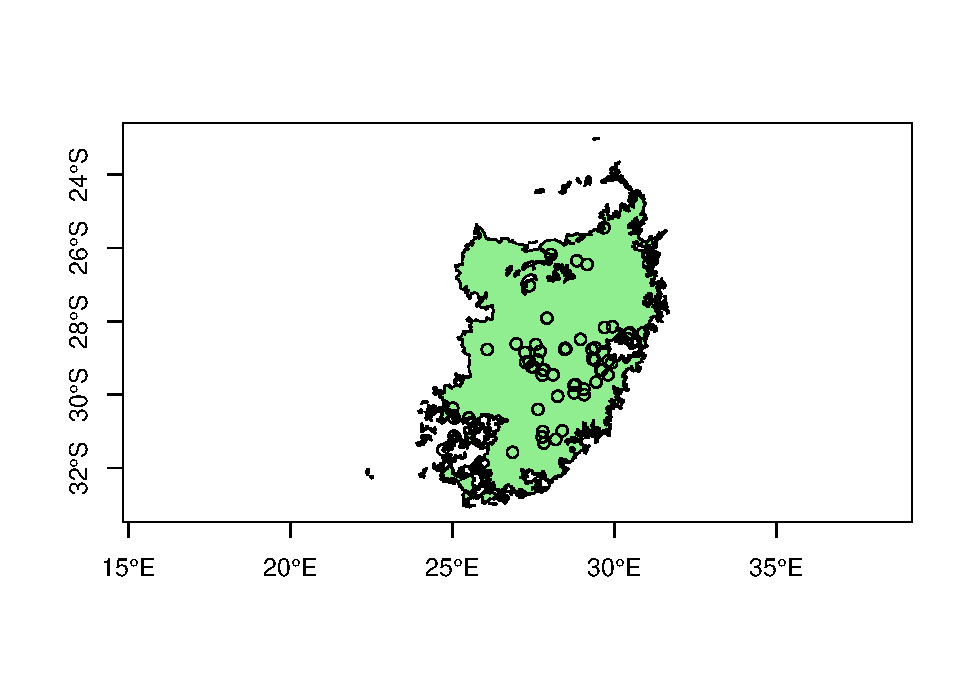
\includegraphics{_main_files/figure-latex/unnamed-chunk-23-1.pdf}

Just looking at this pattern, we can see that some quadrats have more than 100 observations, while others have none at all. This suggests intuitively that the distribution of is patterned, but we can estimate whether this is meaningful using \texttt{quadrat.test}.

\begin{Shaded}
\begin{Highlighting}[]
\FunctionTok{quadrat.test}\NormalTok{(p, }\DecValTok{8}\NormalTok{, }\DecValTok{8}\NormalTok{)}
\end{Highlighting}
\end{Shaded}

\begin{verbatim}
## Warning: Some expected counts are small; chi^2 approximation may be inaccurate
\end{verbatim}

\begin{verbatim}
## 
##  Chi-squared test of CSR using quadrat counts
## 
## data:  p
## X2 = 11974, df = 49, p-value < 2.2e-16
## alternative hypothesis: two.sided
## 
## Quadrats: 50 tiles (irregular windows)
\end{verbatim}

Note that the p-value is \textless{} 2.2e-16. This means that the

\hypertarget{kernel-density-estimation}{%
\section{Kernel Density Estimation}\label{kernel-density-estimation}}

We can visualize broad scale patterning in our data through a kernel density estimate (KDE). This is similar to the above approaches in that it calculates the number of of instances

\begin{Shaded}
\begin{Highlighting}[]
\NormalTok{ecDensity }\OtherTok{\textless{}{-}} \FunctionTok{density}\NormalTok{(p)}
\FunctionTok{plot}\NormalTok{(ecDensity,}\AttributeTok{main=}\StringTok{"Primate Observation Density"}\NormalTok{)}
\FunctionTok{plot}\NormalTok{(p,}\AttributeTok{add=}\NormalTok{T)}
\end{Highlighting}
\end{Shaded}

\includegraphics{_main_files/figure-latex/unnamed-chunk-25-1.pdf}

These exercises are meant to introduce you to \texttt{spatstat} and start looking at spatial analysis in R.

\hypertarget{try-it-yourself}{%
\section{Try it yourself}\label{try-it-yourself}}

\texttt{spatstat} comes with some pre-made datasets to test things out with. These are already saved as \texttt{ppp} objects when you call them. Try doing the following:

\begin{itemize}
\tightlist
\item
  Look at nearest neighbor with the \texttt{redwoods} and \texttt{amacrine} datasets
\item
  Create a kernel density estimate from the \texttt{cells} data
\item
  Do a quadrat analysis, including the quadrat test, using the \texttt{nztrees} data
\end{itemize}

\hypertarget{bringing-it-all-together}{%
\chapter{Bringing it all together!}\label{bringing-it-all-together}}

OK, now you've seen how we get started with doing some spatial analysis in \texttt{spatstat}. Like \texttt{sf} and \texttt{terra}, this package has its own quirks and conventions that take some getting used to. For this exercise, see if you can do the following:

\emph{Load in the makiloa\_boundary2.shp and primary\_features.shp files as vector data
}Convert the boundary to an owin object and the features to a point pattern
*Explore the pattern using quadrats, kernel density, and nearest neighbor distance

  \bibliography{book.bib,packages.bib}

\end{document}
